%!TEX root = ../../architekturdokumentation.tex
\chapter{Deployment}
	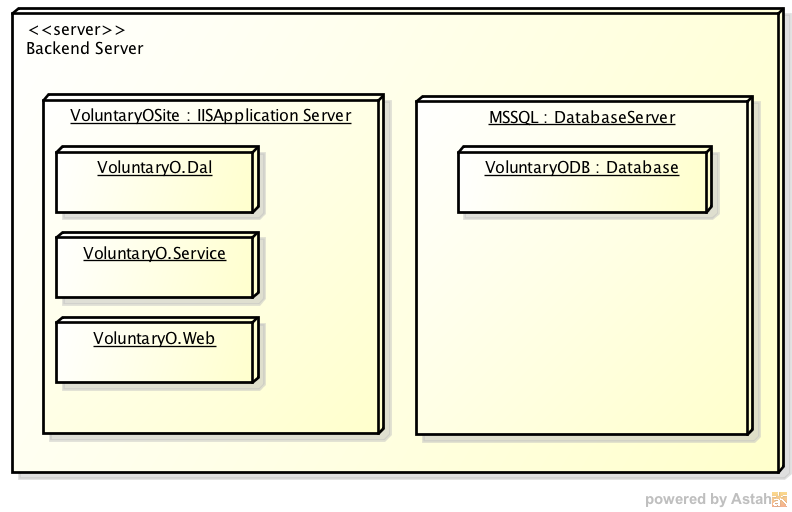
\includegraphics[width=\textwidth]{content/architekturdokumentation/images/DeploymentDiagram.png}
	Die Anwendung besteht aus den Komponenten IIS-Webserver und MSSQL-DB-Server. Für die VoluntaryO-Applikation wird der Datenbankserver auf dem gleichem Server verteilt wie der Applikationsserver. Dies könnte, im Bedarfsfall, dank dem Einsatz des Entity-Frameworks aber leicht geändert werden.

	Für die Entwicklung ist auf jedem Rechner eine eigene Entwicklungsumgebung installiert. Das Deployment von der Entwicklungsumgebun wird über die Visual Studio Funktion Web Deploy angeboten. Auf dem Server läuft der Dienst für Web Deployment, sodass man aus Visual Studio direkt über den Port 80 den Deploymentdienst aufrufen kann.
	Dann wird ein vorkompiliertes Package direkt aus Visual Studio an den Server übertragen. Die Connection Strings zur Datenbank werden direkt im App.Config geändert, sodass auf dem Server die Connection richtig ist.
	Durch diese Konfiguration lässt sich direkt aus Visual Studio mithilfe eines Klicks die gesamte Applikation auf dem Webserver deployen.
	Vor jedem Deploy sollte alle Unit-Tests ausgeführt werden.